%============================================================================
\chapter{Classical black holes}
%============================================================================

%----------------------------------------------------------------------------
\section{Black holes in Einstein gravitation}
%----------------------------------------------------------------------------

\begin{nameddef}{Schwarzschild space-time and black hole}
By inserting a spherical-symmetric ansatz, one obtains the Schwarzschild 
solution of the vacuum Einstein equation. Using the original Schwarzschild 
coordinates and the holonomic formalism, the metric of the solution can be 
written as
\begin{equation}
\dd s^2 = -\rbr{1-\frac{\rSch}{r}}\,\dd t^2+\rbr{1-\frac{\rSch}{r}}^{-1}
\,\dd r^2 + r^2\,\dd\Omega^2,
\label{eq:schwarzschild}
\end{equation}
where $\rSch = 2\nG M$ is the Schwarzschild radius, $M$ can be interpreted 
as the mass of the black hole, and
\begin{equation}
\dd\Omega^2 \coloneqq \dd\theta^2 + \sin^2\theta\,\dd\phi^2
\end{equation}
is the metric of unit $2$-sphere $S^2$. One recognises $0 < \theta < \pp$ and 
$0 < \phi < 2\pp$, whereas $-\infty < t < +\infty$ is also allowed;
the range of $r$ is $\rbr{0, \rSch} \cup \rbr{\rSch, +\infty}$, making the 
coordinates covering two disjoint patches of the space-time.

To exploit the Weyl-flatness of $\mathcal{M}/S^2$, one may transform the
holonomic co-frame by
\begin{equation}
\dd r^* \coloneqq \rbr{1-\frac{\rSch}{r}}^{-1}\,\dd r,
\label{eq:trsf-dtosc}
\end{equation}
which can be integrated to
\begin{equation}
\ee^{r_*/\rSch-1} =
\rbr{\frac{r}{\rSch}-1}\rfun{\exp}{\frac{r}{\rSch}-1},
\label{eq:trsf-gtosc}
\end{equation}
generating the transformations\footnote{$\rfun{W}{x}$ is known as the Lambert 
$W$-function, satisfying $W(x)\ee^{W(x)} = x$}
\begin{equation}
r_* = r+\rSch\rfun{\ln}{\frac{r}{\rSch}-1},\qquad
r = \rSch\rbr{1+\rfun{W}{\ee^{r_*/\rSch-1}}}.
%\label{eq:trsf-scto}
\end{equation}
Transforming by \cref{eq:trsf-dtosc} gives the \emph{Regge and Wheeler's 
tortoise coordinates}, which gives the Schwarzschild metric as
\begin{equation}
\dd s^2 = \rbr{1-\frac{\rSch}{r}}\rbr{ -\dd t^2 + \dd r_*^2}
+ \rfun{r^2}{r_*}\,\dd\Omega^2.
\end{equation}
The range of $r_*$ is $\rbr{-\infty, +\infty}$, corresponding to
$r \in \rbr{\rSch, +\infty}$.

In order to keep the causal structure in further coordinate transformations,
one switches first to the \emph{light-cone} coordinates
\begin{equation}
x_\mp = t\mp r_*.
% u; v
%\\t = \frac{u+v}{2},\quad r_* = \frac{-u+v}{2},
\label{eq:trsf-tlto}
\end{equation}
Substituting $t$ in \cref{eq:schwarzschild} with $x_\mp$ gives
the \emph{retarded and advanced Eddington--Finklestein coordinates}, the 
Schwarzschild metric in which take the form
\begin{align}
\dd s^2
&= -\rbr{1-\frac{\rSch}{r}}\,\dd x_-^2 - 2\,\dd x_-\,\dd r + r^2\,\dd\Omega^2
\label{eq:retarded-efc} \\
&= -\rbr{1-\frac{\rSch}{r}}\,\dd x_+^2 + 2\,\dd x_+\,\dd r + r^2\,\dd\Omega^2,
\label{eq:advanced-efc}
\end{align}
respectively. The ranges of $x_\mp$ and $r$ are now both $\rbr{-\infty, 
+\infty}$. Note that the coordinate singularity at $r=\rSch$ in 
\cref{eq:schwarzschild} has been eliminated.

In \crefrange{eq:retarded-efc}{eq:advanced-efc} one may further replace $r$ 
with $x_\pm$, yielding
\begin{equation}
\dd s^2 = -\rbr{1-\frac{\rSch}{\rfun{r}{x_\mp}}}\,\dd x_-\,\dd x_+
+\rfun{r}{x_\mp}^2\,\dd\Omega^2,
\label{eq:co-sctlo}
\end{equation}
at the expense of recovering the coordinate singularity at $r = \rSch$. To 
bypass this, using
\cref{eq:trsf-gtosc,eq:trsf-tlto} to get
\begin{equation}
1-\frac{\rSch}{r} = \frac{\rSch}{r}\rfun{\exp}{-\frac{r}{\rSch}}
\rfun{\exp}{\frac{-x_-+x_+}{2\rSch}},
\end{equation}
so \cref{eq:co-sctlo} becomes
\begin{equation}
\dd s^2 = -\frac{\rSch}{r}\rfun{\exp}{-\frac{r}{\rSch}}
\rfun{\exp}{\frac{-x_-+x_+}{2\rSch}}\,\dd x_-\,\dd x_+
+ r^2\,\dd\Omega^2.
\end{equation}
Absorbing the corresponding exponentials by introducing the
\emph{Kruskal--Szekeres} light-cone coordinates,
\begin{equation}
X_- \coloneqq -\rSch \rfun{\exp}{-\frac{x_-}{2\rSch}},
\qquad
X_+ \coloneqq +\rSch \rfun{\exp}{+\frac{x_+}{2\rSch}},
\end{equation}
leads to the new components
\begin{equation}
\dd s^2 = 
-\frac{4\rSch}{\rfun{r}{X_\mp}}\rfun{\exp}{-\frac{\rfun{r}{X_\mp}}{\rSch}}
\,\dd X_-\,\dd X_+ + \rfun{r}{X_\mp}^2\,\dd\Omega^2.
\end{equation}
By further rotating the light-cone coordinates into time- and space-like ones,
\begin{equation}
X_- \eqqcolon T-R,\qquad X_+ \eqqcolon T+R,
\end{equation}
one derives the \emph{Kruskal--Szekeres coordinates}, the metric in which takes 
the form
\begin{equation}
\dd s^2 = 
\frac{16\rSch}{\rfun{r}{T,R}}\rfun{\exp}{-\frac{\rfun{r}{T,R}}{\rSch}}
\rbr{-\dd T^2 + \dd R^2} + \rfun{r}{T,R}^2\,\dd\Omega^2.
\end{equation}

Finally, in order to compactify the coordinates $T$ and $R$ while keeping the 
causal structure, one may introducing the \emph{conformal} coordinates of type 
light-cone and space-time
\begin{equation}
\chi_- \coloneqq \arctan\frac{X_-}{\rSch} \eqqcolon \eta - \rho, \qquad
\chi_+ \coloneqq \arctan\frac{X_+}{\rSch} \eqqcolon \eta + \rho,
\end{equation}
leading to the components
\begin{align}
\dd s^2
&= -\frac{4\rSch^3}{r}\ee^{-r/\rSch}\sec^2\chi_-\sec^2\chi_+ 
\,\dd\chi_-\,\dd\chi_+ + r^2\,\dd\Omega^2 \\
&= \frac{16\rSch^3}{r}\ee^{-r/\rSch}
\rfun{\sec^2}{\eta-\rho}\rfun{\sec^2}{\eta+\rho}
\rbr{-\dd\eta^2+\dd\rho^2} + r^2\,\dd\Omega^2.
\end{align}
This leads to the Carter--Penrose conformal diagram of the maximally extended
Schwarzschild space-time, \cref{fig:e-schwarzschild}.

\begin{figure}
\begin{center}
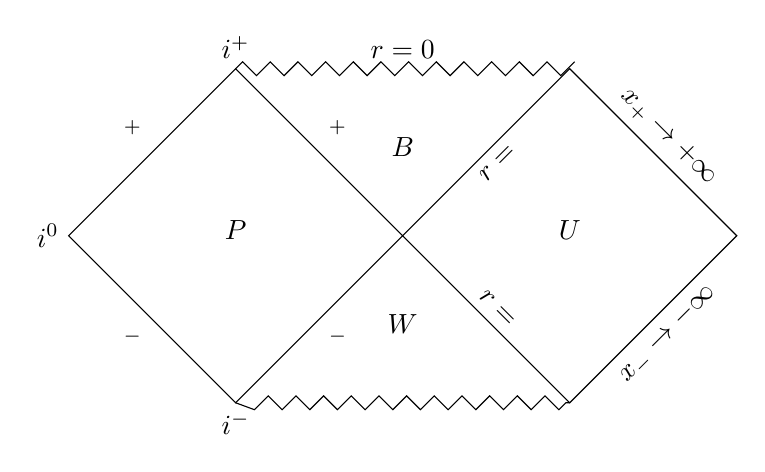
\begin{tikzpicture}%[scale=2]
\pgfmathsetmacro\myunit{3} 
	\draw (0,0)
			node [left] {$i^0$} 
		--++(45:\myunit)
			node [above]{$i^+$}
			coordinate (a)
			node [below = 1.8 cm] {$P$}
			node [pos = .5, above left] {$\mscrI^+$}
			% node [pos=.5, below, sloped] {$\bar{u}=\infty$}
		--++(-45:2*\myunit)
			node [pos = .25, above right] {$\mscrH^+$}
			node [pos = .75, above, sloped] {$r = \rSch$}%x_+ \to -\infty$}
			coordinate (d)	
			%node [below]{$i^-$}
		--++(45:\myunit)
			node [pos = .5, below, sloped] {$x_- \to -\infty$}
			% node [right] {$i^0$}
		--++(135:\myunit)
			% node [above] {$i^+$}
			node [below = 1.8 cm] {$U$}
			coordinate (b)
			node [pos = .5, above, sloped] {$x_+ \to +\infty$}
		--++(-135:2*\myunit)
			coordinate (c)
			node [pos = .25, below, sloped] {$r = \rSch$}%x_- \to +\infty$}
			node [pos = .75, below right] {$\mscrH^-$}
			node [below] {$i^-$}
		--cycle
			node [pos = .5, below left] {$\mscrI^-$};

 \draw [decorate, decoration=zigzag] (a) -- node [above] {$r=0$} % =6pt
											node [below = .75 cm] {$B$}
											(b) 

									 (c) -- node [above = .75 cm] {$W$}
											(d);

\end{tikzpicture}
\end{center}
\caption[Conformal diagram of the Schwarzschild space-time]{Carter--Penrose 
conformal diagram of the maximally extended Schwarzschild space-time, where 
$\pm$ means future and past, $\mscrI^\pm$ denote the light-like infinities, 
$i^0$ the space-like infinity, $i^\pm$ the time-like infinities, and 
$\mscrH^\pm$ the horizons, respectively. $B$, $U$, $W$ and $P$ denote different 
regions, meaning black hole, universe, white hole and parallel universe, 
respectively. The space-time structures of $P$ and $U$ are equivalent. 
\label{fig:e-schwarzschild}}
\end{figure}

\begin{table}
\begin{tabular}{l|l@{,}l|l}
\toprule
Name & & \\
\midrule
Space-time Sch.\ & $t \in \BbbR$ & $r \in \BbbR^+\backslash \cbr{\rSch}$
	& $U\cup B$\\
Space-time R--W & $t \in \BbbR$ & $r_* \in \BbbR$ & $U$\\
Light-cone R--W & \multicolumn{2}{l}{$x_\mp \in \BbbR$} & $U$\\
Retarded E--F & \\
Advanced E--F & \\
Space-time K--S & \\
Light-cone K--S & \\
Space-time Con & \\
Light-cone Con & \\
\bottomrule
\end{tabular}
\caption{Range and valid region of different coordinates}
\end{table}



\end{nameddef}



\begin{nameddef}{Further Einsteinian black holes}

\end{nameddef}



\begin{nameddef}{Collapsing body}

\end{nameddef}


%----------------------------------------------------------------------------
\section{Black holes in dilaton gravitation}
%----------------------------------------------------------------------------

%----------------------------------------------------------------------------
\section{Thermodynamics of Einsteinian black holes}
%----------------------------------------------------------------------------

\begin{nameddef}{Laws of Einsteinian black-hole mechanics}

\end{nameddef}


